
\section{Results}\label{sec:hmmResults}
\subsection{Significance}

The observed data is fit with the B-only and S+B models.
The event multiplicity in the invariant-mass range $\muu\in[120,130]$~GeV is of principle interest, as this region contains the majority of the VH produced events.
The observed yields are provided in Table \ref{tab:hmmResultNdat}.
The number of expected background events, based on the B-only model fit in the invariant-mass sidebands $\muu\in[110,120]\cup[130,160]$, is listed as well.
The first observation is of the excesses of observed events over the expected events in the inclusive 4-lepton and 3-lepton categories.
These excesses are preserved in the post-cut exclusive categories, with a particular excess in the 4-lepton high purity category.
It is interesting to note that the subsequent measurement by CMS found a similar excess in leptonic VH events\cite{cmsHmm}. 

\begin{table}[htp]
\caption{
Yields of data and expected background counted in invariant-mass range $\muu\in[120,130]$~GeV, corresponding to 139 fb$^{-1}$ of integrated luminosity.
The uncertainties on the background estimate are described in Section \ref{sec:hmmBkgUncert}.
}
\begin{center}
\begin{tabular}{l r r r r r}\toprule
Category               & Data    & Background \\
\midrule
4-Lepton               & 51      & 44.5$\pm$2.7 \\
3-Lepton               & 437     & 402.3$\pm$21.0 \\
\midrule
4-Lepton High-Purity   & 34      & 19.1$\pm$1.5 \\
3-Lepton High-Purity   & 41      & 34.2$\pm$2.3 \\
3-Lepton Middle-Purity & 358     & 329.7$\pm$18.7 \\
\bottomrule\end{tabular}\\
\label{tab:hmmResultNdat}
\end{center}
\end{table}

The significances of these observations under the background-only hypothesis are given in Table \ref{tab:hmmSignificance}.
The top of the table shows these for the inclusive categories, while the bottom shows values for the exclusive categories.
The exclusive and inclusive significance are separated to emphasize that these observations are correlated.
Also listed are the probabilities (p-values) to observe a result more incompatible than the observation, supposing the background-only hypothesis.
The p-values are calculated with a frequentist approach. 
An ensemble of 100,000 statistical toys are used to estimate the likelihood of observations under the background-only hypothesis with ensembles of statistical toys.

\begin{table}[htp]
\caption{Significance and p-values of the observed data yield in $\muu\in[120,130]$~GeV given the expected background.}
\begin{center}
\begin{tabular}{l r r r r r}\toprule
Category & Significance $\sigma$ & p-value \\
\midrule
3-Lepton & 0.75 & 0.23 \\
4-Lepton & 0.70 & 0.24 \\
\midrule
4-Lepton High Purity & 2.47 & 0.01 \\
3-Lepton High Purity & 0.83 & 0.20 \\
3-Lepton Middle Purity & 0.69 & 0.25 \\
\bottomrule\end{tabular} %remember cline{1-2}
\label{tab:hmmSignificance}
\end{center}
\end{table}

The largest significance is that of the observation in the 4-lepton High-Purity category, approaching 2.5$\sigma$.
The combined significance of observations in the inclusive 4-lepton and 3-lepton categories is $1.03\sigma$.
As a result of the higher sensitivity of the exclusive categories, the exclusive observations have a combined significance of $2.70\sigma$.
These observations can be compared to two similar observations.
First, the CMS collaboration has reported a significance in their leptonic VH \hmm observation with a significance of 2.02$\sigma$ \cite{cmsHmm}.
Other observations by the ATLAS experiment have been made for VH production in different Higgs boson decay channels: $\gamma\gamma$, $\Z\Z$, and $b\bbar$.
These previous observations all report a modest excesses of events that is compatible at a level of $\approx1\sigma$ with the Standard Model prediction \cite{atlashiggs}.


\subsection{Limits}

The observed invariant-mass distributions are shown in Figures \ref{fig:hmmFits}.
The S+B model (Equation \ref{eqn:hmmSbFunc}) and B-only (Equation \ref{eqn:hmmBkgFunc}) models, fit to the data, are shown.
The excesses of events shown in Table \ref{tab:hmmResultNdat} results in positive measurements of the signal strength, \mus, in each category.


\afterpage{
\begin{figure}[htp]
\captionsetup[subfigure]{position=b}
\centering
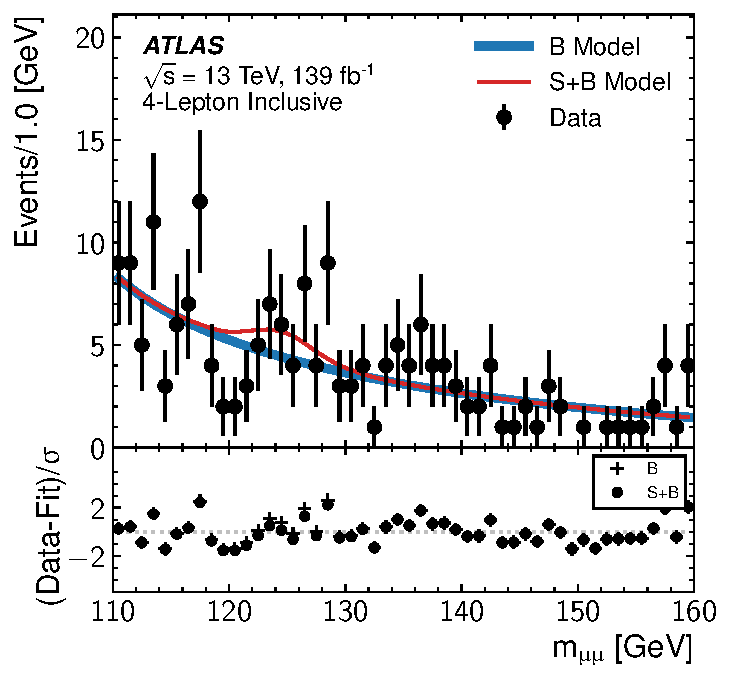
\includegraphics[width=0.45\textwidth]{figures/hmm/fitData2/ratio-4lep-dat.pdf}
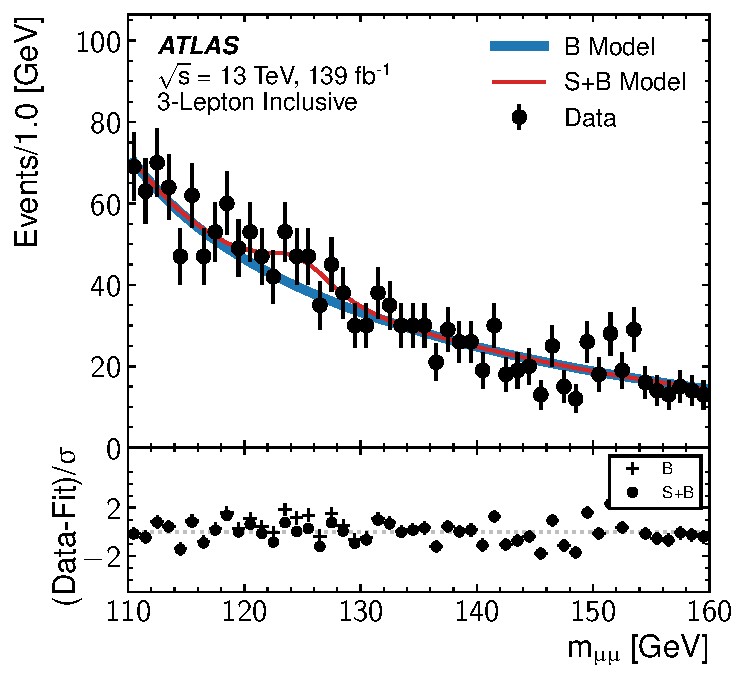
\includegraphics[width=0.45\textwidth]{figures/hmm/fitData2/ratio-3lep-dat.pdf}\\
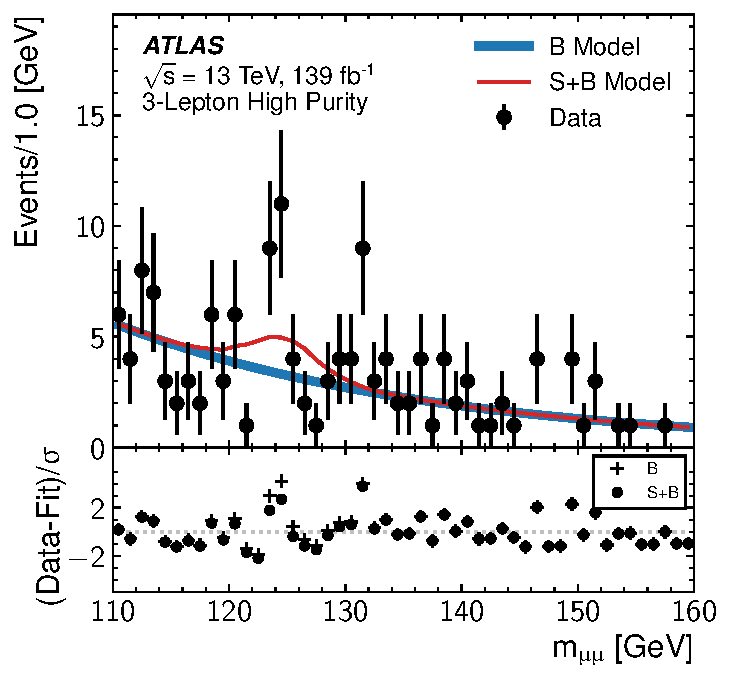
\includegraphics[width=0.45\textwidth]{figures/hmm/fitData2/ratio-3lep0-dat.pdf}
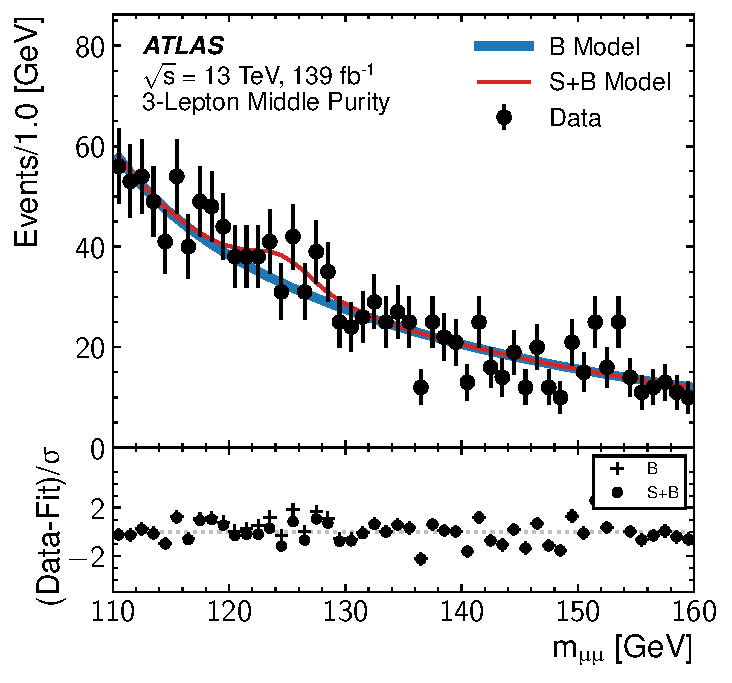
\includegraphics[width=0.45\textwidth]{figures/hmm/fitData2/ratio-3lep1-dat.pdf}\\
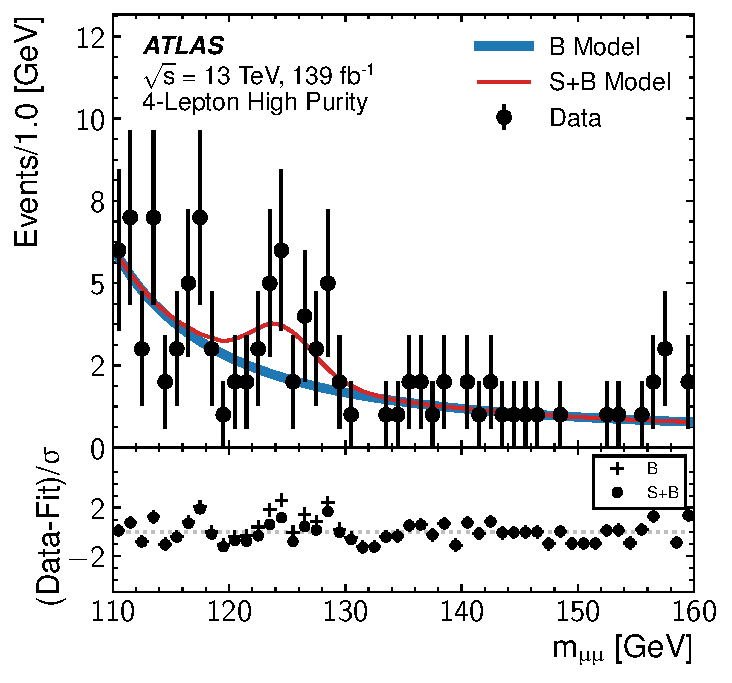
\includegraphics[width=0.45\textwidth]{figures/hmm/fitData2/ratio-4lep0-dat.pdf}
\caption{The S+B (red) and B-only (blue) models fit to data (black).}
\label{fig:hmmFits}
\end{figure}
\clearpage
}


% \begin{figure}[htp]
% \captionsetup[subfigure]{position=b}
% \centering
% \subfloat[][]{{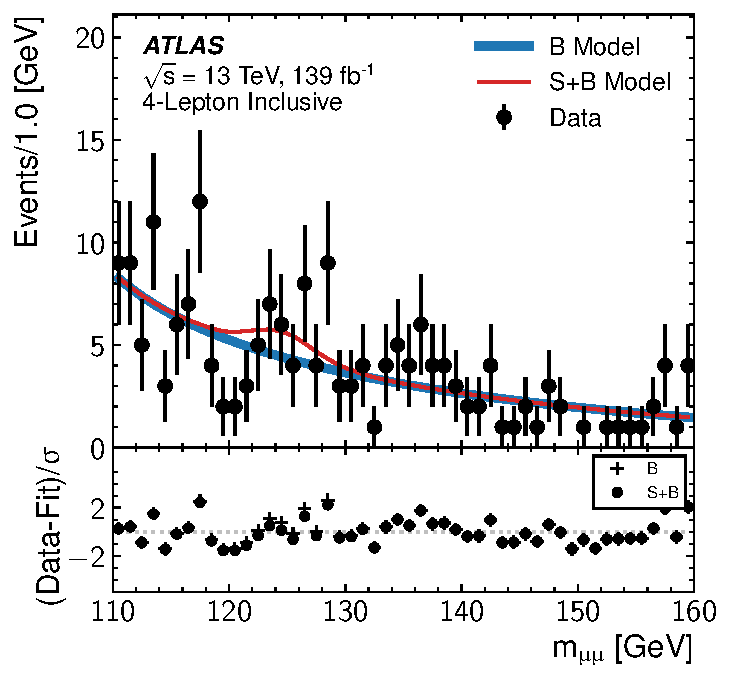
\includegraphics[width=0.5\textwidth]{figures/hmm/fitData2/ratio-4lep-dat.pdf}}}
% \subfloat[][]{{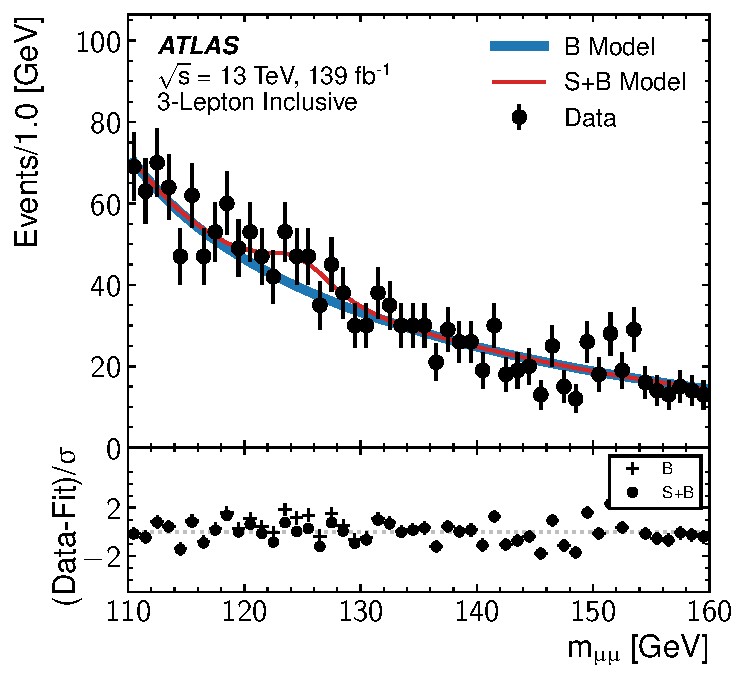
\includegraphics[width=0.5\textwidth]{figures/hmm/fitData2/ratio-3lep-dat.pdf}}}
% \caption{Fits of the S+B and B-only models to the data observed in the inclusive 4-lepton (a) and 3-lepton (b) categories.}
% \label{fig:hmmPrecutFits}
% \end{figure}

% \begin{figure}[htp]
% \captionsetup[subfigure]{position=b}
% \centering
% \subfloat[][]{{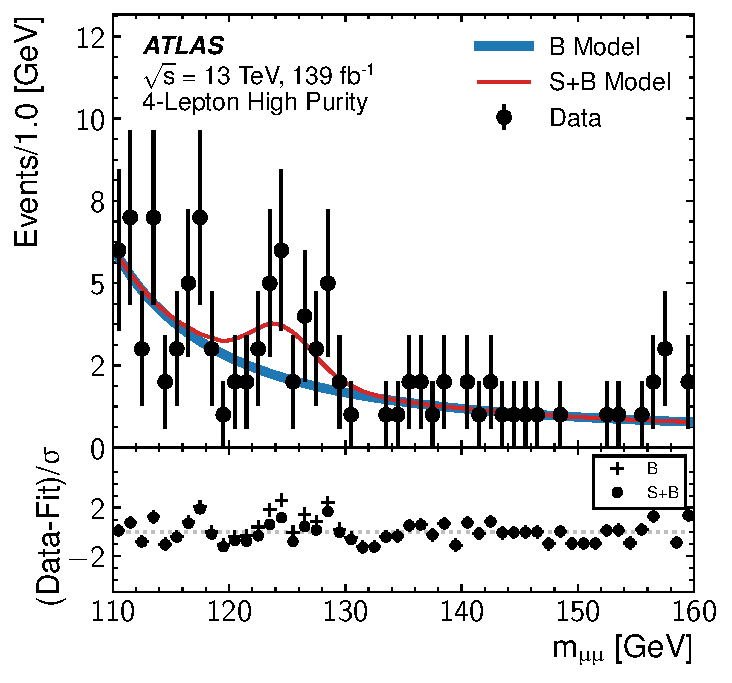
\includegraphics[width=0.5\textwidth]{figures/hmm/fitData2/ratio-4lep0-dat.pdf}}}\\
% \subfloat[][]{{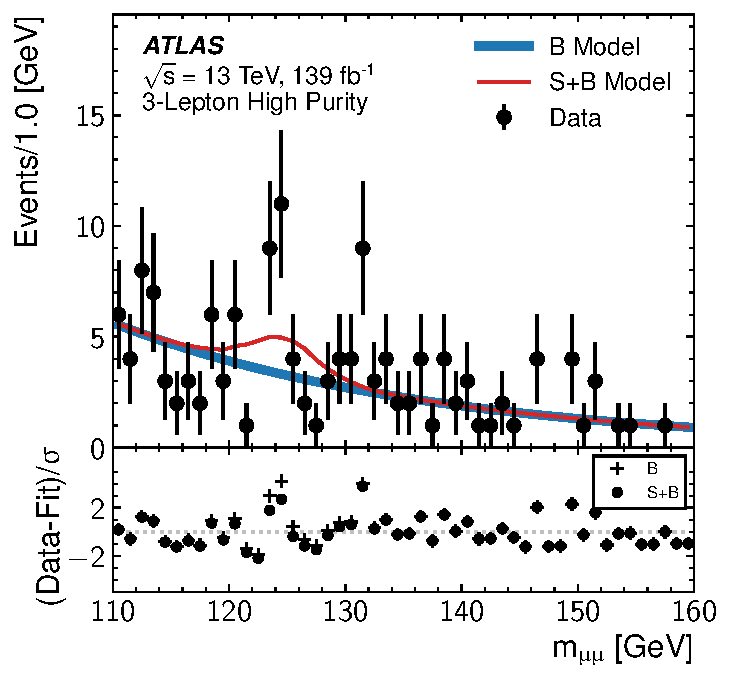
\includegraphics[width=0.5\textwidth]{figures/hmm/fitData2/ratio-3lep0-dat.pdf}}}
% \subfloat[][]{{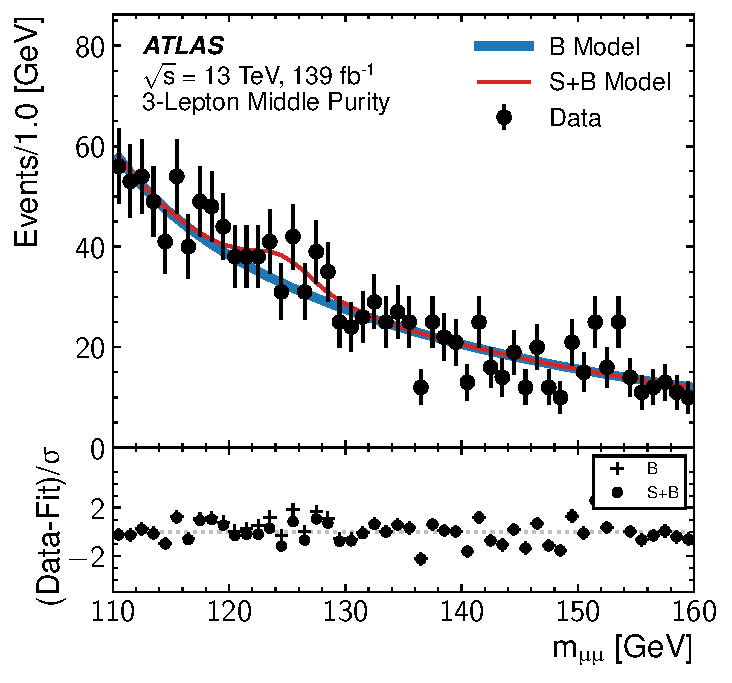
\includegraphics[width=0.5\textwidth]{figures/hmm/fitData2/ratio-3lep1-dat.pdf}}}
% \caption{Fits of the S+B and B-only models to the data observed in the exclusive 4-lepton high-purity (a), 3-lepton high-purity (b), and 3-lepton middle-purity categories.}
% \label{fig:hmmPostcutFits}
% \end{figure}

% \begin{table}[htp]
% \caption{Asymptotic upper limits set at 95\% confidence levels on the signal strength \mus in each of the inclusive (top) and exclusive (bottom) categories. The signal strength corresponds to a number of signal events $N_S$, and these are provided as well.}
% \begin{center}
% \begin{tabular}{l r r r r r }
% \toprule
% \multirow{2}{*}{Category} & \multicolumn{2}{c}{Limit on $N_S$} & & \multicolumn{2}{c}{Limit on \mus} \\
% \cline{2-3} \cline{5-6} 
% & Expected & Observed & & Expected & Observed \\
% \midrule
% 3-Lepton & 63.7 & 112.5 & &  13.2 & 22.6 \\
% 4-Lepton & 23.2 & 30.1 & &  33.2 & 42.8 \\
% \midrule
% 4-Lepton High-Purity & 14.7 & 28.3 & &  23.7 & 45.1 \\
% 3-Lepton Middle-Purity & 58.1 & 94.4 & &  18.7 & 29.8 \\
% 3-Lepton High-Purity & 20.6 & 29.5 & &  12.0 & 17.2 \\
% \bottomrule
% \end{tabular}
% \label{tab:hmmLimits}
% \end{center}
% \end{table}


The observed data shown in these figures restrict the plausibility of signal production mechanisms that predict events produced in the range $\muu\in[110,160]$.
Exclusion limits are set on the largest signal mechanisms that retain compatibility with the data.
The Standard Model VH \hmm production, scaled by a coefficient \mus, is used as a set of benchmark signal models for this purpose.
These limits are set in the fiducial volume defined in Section \ref{sec:hmmEv}, in the invariant-mass range $\muu\in[110,160]$.
They apply to the production of Higgs-like signal events in the inclusive and exclusive categories.

\begin{table}[H]
\caption{Upper limits set at 95\% confidence levels on the signal strength \mus in each of the inclusive (top) and exclusive (bottom) categories. The signal strength corresponds to a number of signal events $N_S$, and these are provided as well. These frequentist limits are set with $\approx$ 50,000 toys.}
\begin{center}
\begin{tabular}{l r r r r r }
\toprule
\multirow{2}{*}{Category} & \multicolumn{2}{c}{Upper limit on \nsig} & & \multicolumn{2}{c}{Upper limit on \mus} \\
\cline{2-3} \cline{5-6} 
& Expected & Observed & & Expected & Observed \\
\midrule
3-Lepton & 52.9 & 110.3 & & 10.7 & 22.2 \\
4-Lepton & 17.1 & 30.1 & & 24.3 & 42.6 \\
\midrule
4-Lepton High Purity & 12.7 & 29.0 & & 20.3 & 46.1 \\
3-Lepton High Purity & 16.0 & 29.7 & & 9.3 & 17.3 \\
3-Lepton Middle Purity & 47.0 & 92.4 & & 14.9 & 29.2 \\
\bottomrule
\end{tabular}
\label{tab:hmmLimits}
\end{center}
\end{table}

% inclusive
The top half of Table \ref{tab:hmmLimits} reports limits set at 95\% confidence level in the inclusive categories.
The fiducial volumes for the inclusive categories specify a multi-lepton phase space but do not detailed further requirements on the kinematic character of a potential signal.
This makes these limits relatively model-independent and interpretable in terms of other signal production mechanisms.
For this purpose, the limits are provided both on the signal strength \mus for the Standard Model VH, and in terms of the number of signal events, \nsig.

% exclusive
The bottom half of the Table \ref{tab:hmmLimits} presents limits set in the exclusive categories.
The use of the MVA discriminant in the case of the exclusive categories means that these limits are only applicable to signal models with the same kinematic distributions as the Standard Model Higgs. 
For these, the limits on the Standard Model signal strength are most relevant.

The limits on the \nsig are equivalent to limits on the visible cross-section times branching ratio, \xsbr, times the dataset luminosity.
In all cases, the excesses reported in Table \ref{tab:hmmResultNdat} result in weaker observed limits than expected.
The particularly large excess observed in the 4-lepton high purity category raises the observed limit to over twice the expected limit.

\subsection{Other production mechanisms}

The observations made in the three exclusive VH categories are included in a combined search for \hmm that includes categories targeting additional production mechanisms.
In particular, a superset of the VH event selection identifies events with at least dimuon pair.
Events with a b-jet are identified as ttH candidates.
Events with two jets and a kinematic profile that matches simulated VBF production are identified as VBF candidates.
The remaining events are ggH candidates and are separated into zero, one, and two jet categories.
Each category is separated into four sub-categories using an MVA discriminant.
The composition and purity of these categories are illustrated in Figure \ref{fig:hmmComb}.
\cite{atlasHmm}

The combined categories are used to set limits at 95\% confidence on the Standard Model production of \hmm events.
The observed (expected) limit is 2.0 (1.7) times the Standard Model cross-section times branching ratio, reflecting an overall excess of observed events over the background prediction in the signal region.
This provides a strong hint of the \hmm production at the LHC.

\afterpage{
\begin{figure}[h!]
\captionsetup[subfigure]{position=b}
\centering
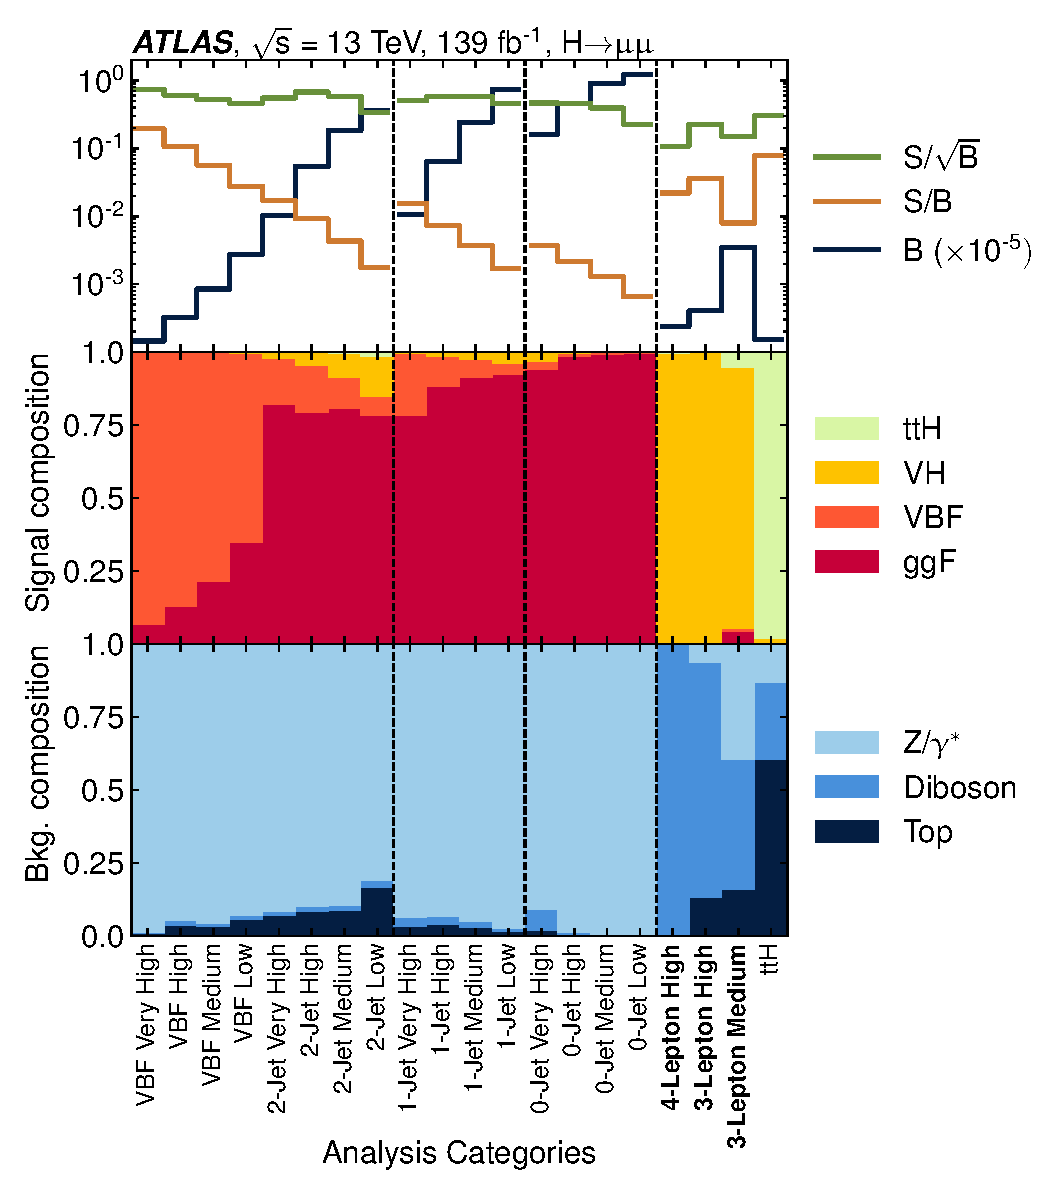
\includegraphics[width=0.99\textwidth]{figures/hmm/comb/Categorisation_.pdf}
\caption{
Overview of the signal and background compositions in the twenty analysis categories used in the combined \hmm search.
The VH categories are indicated in bold text.
Each quantity is calculated in $\mh\in[120,130]$~GeV based on simulation.
(Top) Ratios of signal to background yields. 
(Middle) Relative signal compositions.
(Bottom) Relative background compositions.
}
\label{fig:hmmComb}
\end{figure}
\clearpage
}

\subsection{Summary}

This chapter presented a search for the rare decay of the Standard Model Higgs boson to two muons using the VH production channels.
This search is challenging on two accounts.
First, tiny branching fraction of the Higgs boson to muons limits the production of events from such production mechanisms.
Second, the large irreducible background of dimuon events serves to mask the rare signal events.
A new strategy is adopted to use the leptonic final state of VH production.
The additional leptons in the final state are used to separate VH events from the Drell-Yan, diboson, and top backgrounds.
This particular phase space previously had not been investigated by either the ATLAS or CMS collaborations.

Identifying events from \vhmm production is complicated by the small leptonic branching ratio of the \W and \Z bosons.
However, making use of the additional kinematic information from the leptons yields a powerful lever to further reduce backgrounds.
% Techniques to address challenge
A new set of selection criteria captures as many VH events as possible.
Machine-learning methods in the form of a multivariate analysis discriminant are used to take advantage of the kinematic information from the W/Z decays.
Careful use of k-fold splitting and test/validation/train designations are introduced to avoid introducing uncontrolled bias.

Moderate excesses are seen above the expected number of events in the three and four lepton categories.
In the inclusive categories the observations remain compatible with the background-only hypothesis.
The combined significance of the inclusive observations is 1.03$\sigma$.
In the more sensitive exclusive categories, tension is observed in the 4-lepton high purity category and not in the others.
% No significant departure from the expected background is observed in data.
Limits are set on VH Higgs-like signal hypotheses.
The strongest expected (observed) limit on leptonic VH production excludes signals down to 10.8 (22.3) times the Standard Model prediction.
These limits are the first to be set in this particular phase space.
Limits are set on the numbers of signal events in 3-lepton and 4-lepton fiducial volumes.
These exclude the visible cross-section times branching ratio those regions above \xsbr=0.39~fb and \xsbr=0.22~fb, respectively.
